\documentclass[11pt,a4paper,dvipdfmx]{article}
%\documentclass[autodetect-engine,dvipdfmx-if-dvi,ja=standard]{bxjsarticle}

\usepackage[utf8]{inputenc}
\usepackage{lmodern}
\usepackage[T1]{fontenc}
\usepackage[noBBpl]{mathpazo}
%\linespread{1.05}
\usepackage{mathtools, amsmath, amssymb, amsthm}
\usepackage{amsfonts}
\usepackage{braket}
%\usepackage{amssymb}
\usepackage{url}
\usepackage{cases}

%% citation
\usepackage[longnamesfirst]{natbib}

%
\theoremstyle{plain}
\newtheorem{thm}{Thm.}[section]
\newtheorem{lem}{Lem.}[section]
\newtheorem{cor}{Cor.}[section]
\newtheorem{prop}{Prop.}[section]
\newtheorem{df}{Def.}[section]
\newtheorem{eg}{e.g.}[section]
\newtheorem{rem}{Rem.}[section]
%

\usepackage{listings}
\lstset{%
language={python},%
basicstyle={\ttfamily\footnotesize},%ソースコードの文字を小さくする
frame={single},
commentstyle={\footnotesize\itshape},%コメントアウトの文字を小さくする
breaklines=true,%行が長くなったときの改行。trueの場合は改行する。
numbers=left,%行番号を左に書く。消す場合はnone。
xrightmargin=3zw,%左の空白の大きさ
xleftmargin=3zw,%右の空白の大きさ
stepnumber=1,%行番号を1から始める場合こうする(たぶん)
numbersep=1zw,%行番号と本文の間隔。
}

%\usepackage[dvipdfmx]{graphicx}
%% color packageとdvipdfmxは相性が悪いらしい
%% https://qiita.com/zr_tex8r/items/442b75b452b11bee8049
\usepackage{graphicx}


\usepackage[left=2cm,right=2cm,top=2cm,bottom=2cm]{geometry} %This changes the margins.
\usepackage{float}
%\author{Kyohei Okumura}
\global\long\def\T#1{#1^{\top}}

\newcommand{\id}{\textnormal{id}}
\newcommand{\R}{\mathbb{R}}
\newcommand{\N}{\mathbb{N}}
\newcommand{\Q}{\mathbb{Q}}
\newcommand{\Z}{\mathbb{Z}}
\newcommand{\C}{\mathbb{C}}
\newcommand{\mF}{\mathcal{F}}
\newcommand{\mG}{\mathcal{G}}
\newcommand{\mA}{\mathcal{A}}
\newcommand{\mB}{\mathcal{B}}
\newcommand{\mC}{\mathcal{C}}
\newcommand{\mD}{\mathcal{D}}
\newcommand{\mL}{\mathcal{L}}
\newcommand{\mM}{\mathcal{M}}
\newcommand{\mO}{\mathcal{O}}
\newcommand{\mP}{\mathcal{P}}
\newcommand{\mS}{\mathcal{S}}
\newcommand{\mT}{\mathcal{T}}
\newcommand{\mV}{\mathcal{V}}
\renewcommand{\Re}{\mathrm{Re}}
\renewcommand{\hat}{\widehat}
\renewcommand{\tilde}{\widetilde}
\renewcommand{\bar}{\overline}
\renewcommand{\epsilon}{\varepsilon}
% \renewcommand{\span}{\mathrm{span}}
\newcommand{\defi}{\stackrel{\Delta}{\Longleftrightarrow}}
\newcommand{\equi}{\Longleftrightarrow}
\newcommand{\s}{\succsim}
\newcommand{\p}{\precsim}
\newcommand{\join}{\vee}
\newcommand{\meet}{\wedge}
\newcommand{\1}{\mbox{1}\hspace{-0.25em}\mbox{l}}

\DeclareMathOperator{\Var}{Var}
\DeclareMathOperator{\Cov}{Cov}
\DeclareMathOperator{\sgn}{sgn}
\DeclareMathOperator{\Card}{Card}
\DeclareMathOperator{\supp}{supp}
\DeclareMathOperator{\Log}{Log}
\DeclareMathOperator{\spn}{span}

\newcommand{\indep}{\mathop{\perp\!\!\!\!\perp}}

\usepackage{color}
\newcommand{\kcomment}[1]{{\textcolor{blue}{#1}}}
\newcommand{\ocomment}[1]{{\textcolor{red}{#1}}}


\begin{document}
\title{SML HW5}
\author{29-176004 奥村 恭平{\footnote{E-mail: kyohei.okumura@gmail.com}
\footnote{東京大学大学院 経済学研究科 M2}
}}
\date{\today}
\maketitle

%%%%%%%%%%%%%%%%%%%%%%%%%%%%%%%%%%%%%%%%%%%%%%%%%%%%%%%%%%%

\section*{宿題1: $\tilde{M}$が直交行列になることを示せ}
$$
\tilde{M}^\top \tilde{M} = I_d
$$
を示せば十分.
$\tilde{M} = C^{-\frac{1}{2}}M$より,
\begin{align*}
	\tilde{M}^\top \tilde{M} &= M^\top C^{-1} M \\
	&= M^\top \left( \frac{1}{n} \sum_i x_i x_i^\top \right)^{-1} M \\
	&= M^\top \left( \frac{1}{n} X X^\top \right)^{-1} M \quad (X := (x_1, \dots, x_n) \text{とした}) \\
	&= n M^\top \left(  X X^\top \right)^{-1} M
\end{align*}
ここで,
$
M^\top \left(  X X^\top \right)^{-1} M
= (M^{-1} X X^\top (M^\top)^{-1})^{-1} = (S S^\top)^{-1} = (\sum_i s_i s_i^\top)^{-1}
$
(ただし,$S = (s_1, \dots, s_n)$とした) であること,および,$\frac{1}{n}\sum_i s_i s_i^\top = I_d$(原信号に対する仮定)より,

\begin{align*}
	\tilde{M}^\top \tilde{M}
	&= n M^\top \left(  X X^\top \right)^{-1} M \\
	&= n \left( \sum_i s_i s_i^\top \right)^{-1} \\
	&= \left( \frac{1}{n} \sum_i s_i s_i^\top \right)^{-1} \\
	&= I_d
\end{align*}
となる.
\qed

\newpage
\section*{宿題2}
$g(s) = s^3$に対する射影追跡の近似ニュートンアルゴリズムを実装した.言語はpython.以下はシミュレーション結果の図.非ガウス方向を検出できていることがわかる.

\begin{figure}[H]
  \centering
    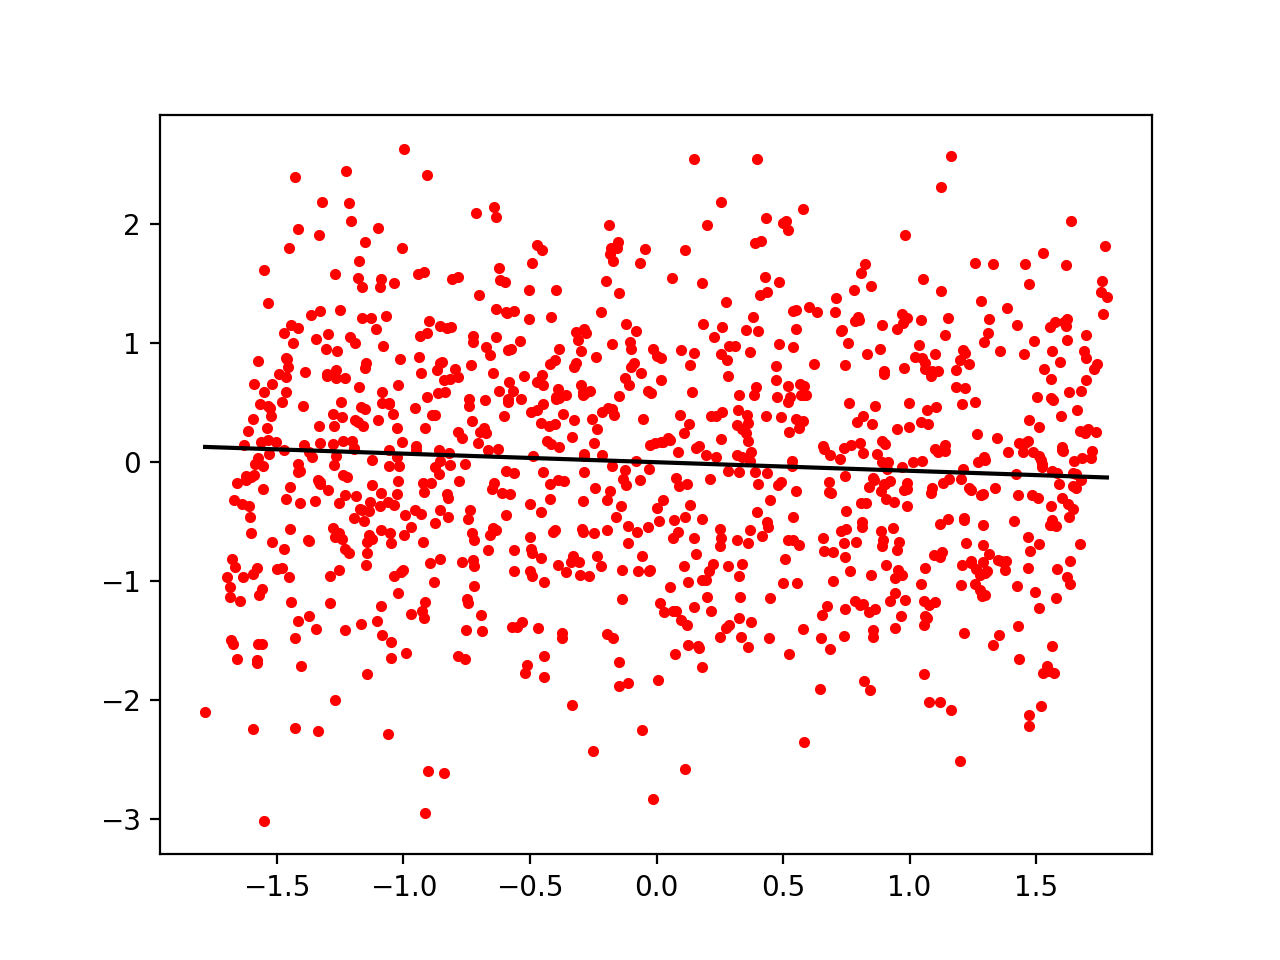
\includegraphics[height=8cm]{image/newton.png}
    \caption{\footnotesize シミュレーション実行結果}
\end{figure}

\begin{lstlisting}
import numpy as np
from scipy.linalg import sqrtm
import matplotlib.pyplot as plt


def centering_sphering(X):
    '''
    X: d x n matrix
    '''
    n = X.shape[1]
    H = np.eye(n) - np.ones((n,n))/n
    XH = np.dot(X, H)
    temp = sqrtm(np.linalg.inv(np.dot(XH, XH.T)/n))
    X_tilde = np.dot(temp, XH)
    return X_tilde


def approx_newton(X, Nlim=50):
    '''
    X should be normalized.
    X: d x n matrix
    '''
    n = X.shape[1]
    b = np.array([1,0])
    threshold = 1e-08
    diff = np.inf
    n_loop = 1
    
    while n_loop < Nlim:
        #print(b)
        b_prev = b
        sum = 0
        for i in range(n):
            sum += X[:, i] * (np.dot(b, X[:, i]) ** 3)
        b = 3 * b - sum/n
        b = b / np.linalg.norm(b)
        diff = np.linalg.norm(b - b_prev)
        if (diff < threshold):
            break
        else:
            n_loop += 1
    
    if n_loop == Nlim:
        print('may not be converged')
    
    return b


def line(b, X):
    x_min = np.min(X[0])
    x_max = np.max(X[0])
    x = np.linspace(x_min, x_max, 1000)
    return [x, (b[1]/b[0])*x]


def plot(x1, line=None):
    x = x1[0]
    y = x1[1]
    plt.plot(x, y, 'ro', ms=3, label='class1')

    if not (line is None):
            plt.plot(line[0], line[1], 'k-', ms=5)
            
    #plt.xlim(np.min(x)-1, np.max(x)+1)
    #plt.ylim(np.min(y)-1, np.max(y)+1)
    
    plt.show()

# simulation
N = 1000

## original sigmal
s_gauss = np.random.randn(N)*2 + 3
s_uniform = np.random.rand(N) * 3 - 2
S = np.array([s_gauss, s_uniform])

## transformation matrix
M = np.array([[1,3],[5,1]])

## observed sigmal
X = np.dot(M, S)

X_tilde = centering_sphering(X)
b = approx_newton(X_tilde)

plot(X_tilde, line(b, X_tilde))

\end{lstlisting}

\end{document}